\documentclass[11pt]{article}
\usepackage[margin=4cm]{geometry}                % See geometry.pdf to learn the layout options. There are lots.
\geometry{letterpaper}                   % ... or a4paper or a5paper or ...
%\geometry{landscape}                % Activate for for rotated page geometry
%\usepackage[parfill]{parskip}    % Activate to begin paragraphs with an empty line rather than an indent
\usepackage{algorithm}
\usepackage[noend]{algpseudocode}
\usepackage{graphicx}
\usepackage{amssymb,amsfonts}
\usepackage{epstopdf}
\usepackage{multicol}
\usepackage{multirow}
\usepackage{tabularx}
\DeclareGraphicsRule{.tif}{png}{.png}{`convert #1 `dirname #1`/`basename #1 .tif`.png}
\setlength\parindent{8mm}
\title{Evacuating Priority Agents in a Disk with Unknown Exit Location}
\author{David Bushta, Christopher Till, Sunil Shende}
%\date{}                                           % Activate to display a given date or no date

\begin{document}
\maketitle
\section{Preliminaries}

\begin{flushleft}
Algorithms of search-and-escape involve mobile agents (also called Robots)
searching in geometric domains, such as a closed disk, or convex polygon. By
working together and communicating with one another, these mobile agents search
the domain to find an exit hidden on the perimeter. Many different problems have
previously been studied in this topic, such as finding algorithms to evacuate all
agents in a domain, or only evacuating a specific subset of these agents.
\end{flushleft}

\subsection{Model}

\begin{flushleft}

All agents in this problem use the same coordinate system and operate in a closed
disk, all starting from the center. These agents' algorithms do not all have to be the same,
and in fact to most efficiently search the circle, they must all be unique.
In our problem, we observe the Priority model of algorithms. In this model, a
subset of one or more agents (P) are defined as a Priority (or Queen) and the goal
of the algorithm is to evacuate a required subset of these Priority Agents. These
algorithms also include a number Helper agents (H), that simply assist in searching the circle
for the exit, for a total of (H + P) agents. The Helper agents are not required to evacuate.


\vspace*{5mm} \hspace{\parindent} Once an exit is found, whether by a Helper or a Priority, the agent may use
Wireless communication to immediately broadcast the exit's location and its own identity to all other agents.
Upon receiving this broadcasted location, any remaining Priority agents that
need to evacuate travel along a chord to the exit and when the required subset has exited, the algorithm terminates.
The cost of the algorithm is called the termination time, and is the total worst-case
time for the required subset of Priority agents to exit.
\end{flushleft}

\subsection{Previous Work}

\begin{flushleft}
Similar search-and-evacuate problems to this one have previously been studied, including those involving Agents
searching on a line, and searching inside of other types of shapes, such as a triangle.
In our research thus far, we have mainly looked at the problems regarding
the closed unit disk and how to most efficiently search for the exit and evacuate
different subsets of agents. We started by studying the algorithms that have been designed
for $n = 2, 3$ agents using both the face-to-face and wireless communication models [(Evacuating Robots
From a Disk Using Face-to-Face Communication, 2015), (Evacuating Robots Via an Unknown Exit in a Disk, 2015)].
In these algorithms, all agents must evacuate for the algorithm to terminate, and there is no notion of
Priority of Helper. Interestingly, in the face-to-face model, agents must be next to each other to
communicate.

\vspace*{5mm} \hspace{\parindent} Afterwards, we looked at problems of a similar type that have been studied,
namely those regarding 1 Priority and 1 or more Helper agents searching in a
closed disk solely usign wireless communication (God Save the Queen, 2018)
(Priority Evacuation From a Disk Using Mobile Robots, 2018)].
In these papers, the results involved getting the only Priority agent to the exit
as fast as possible, however, our problem attempts to design an algorithm where
only one of multiple Priority agents needs to evacuate.

\vspace*{5mm} \hspace{\parindent} To facilitate studying these algorithms and seeing results based on test data, we
have created an algorithm visualizer. This program uses the different types of movement and
communication directives we commonly see in each algorithm to recreate an
interactive visualization of the algorithm. To date, all of the algorithms
listed in the above papers including our own can be shown, and new ones can be created.
\end{flushleft}


\subsection{Our Results}

\begin{flushleft}
\hspace{\parindent} In our initial algorithm using 2 Priority and 1 Helper agent with 1 Priority required to exit, we can show that a termination time
upper bound of \textbf{3.55 time units} is possible given the specific set of parameters we use
to guide the agents. We can achieve this by using a \textbf{parameter of angle $\alpha = 5 \pi / 9 - 2\sqrt3 /3$} for the two agents to travel to the perimeter in the third quadrant, i.e, they travel out at
an angle of \textbf{$\pi + \alpha$}. This allows us to set the two worst-case time predictions equal.
These are the cases where \textbf{$A)$} $P2$ finds the exit at the very end of its search,
or \textbf{$B)$} $H$ finds the exit in the second quadrant at the angle \textbf{$\pi - \beta$},
where \textbf{$\beta = ( \pi / 3 - \alpha) / 2$}.

\hspace{\parindent} As of now, in our second slightly improved algorithm, we predict that we can get a
better time than was shown in the initial algorithm, by making $P1$ take a detour at some point during its
search, leaving it a constant distance away from $H$ during the last phase of its search. By making it
take this detour, we believe that we can improve the upper bound in the case where $P1$ and $P2$ are
equidistant from $H$ at the time when $H$ finds the exit. By using a slightly modified $\alpha$ and introducing some new variables, we believe we can achieve an upper bound of less than 3.55 time units.
\end{flushleft}


%%%%%%%%%%%%%%%%%%%%%%%%%%%%%%%%%%%%%%%%%%%%%%%%%%%%%%%%%%%%%%%%%%%%%%%%%%%%%%%%%%%%%%%
%Marks end of section 1 so that it doesnt make the title of section 2 on the same page%
%If there are issues remove it, it's removed now because the spacing is okay          %
%%%%%%%%%%%%%%%%%%%%%%%%%%%%%%%%%%%%%%%%%%%%%%%%%%%%%%%%%%%%%%%%%%%%%%%%%%%%%%%%%%%%%%%
% \vfill


\section{Initial Algorithm}

\subsection {Evacuation Algorithm \textbf{$Search_{1}$}}

%Our first priority algorithm with 2 queens and 1 servant
\begin{center}
    \begin{tabular}{ | p{1.25cm} || r l | l |}
        \hline
        \multicolumn{4} { | c | }{ Algorithm \textbf{$Search_{1}$}($\alpha$)} \\ \hline
        \textbf{Robot} & $\textbf{\#}$ & \textbf{Trajectory} & \textbf{Exit Protocol} \\ \hline
        \multirow{2}{*}{$P1$} & 0 & Travel from $O$ to $C_{0}$ & IF: Exit found by $P1$ - Done. \\
        & 1 & Travel CCW. & ELSE: Travel along chord to exit if closer. \\  \hline
        \multirow{2}{*}{$P2$} & 0 & Travel from $O$ to $C_{\pi + \alpha}$ & IF: Exit found by $P2$ - Done. \\
        & 1 & Travel CCW. & ELSE: Travel along a chord to exit if closer.\\ \hline
        \multirow{2}{*}{$H$} & 0 & Travel from $O$ to $C_{\pi + \alpha}$ & \multirow{2}{*}{Broadcast exit location and then wait.} \\
        & 1 & Travel CW. & \\ \hline
    \end{tabular}
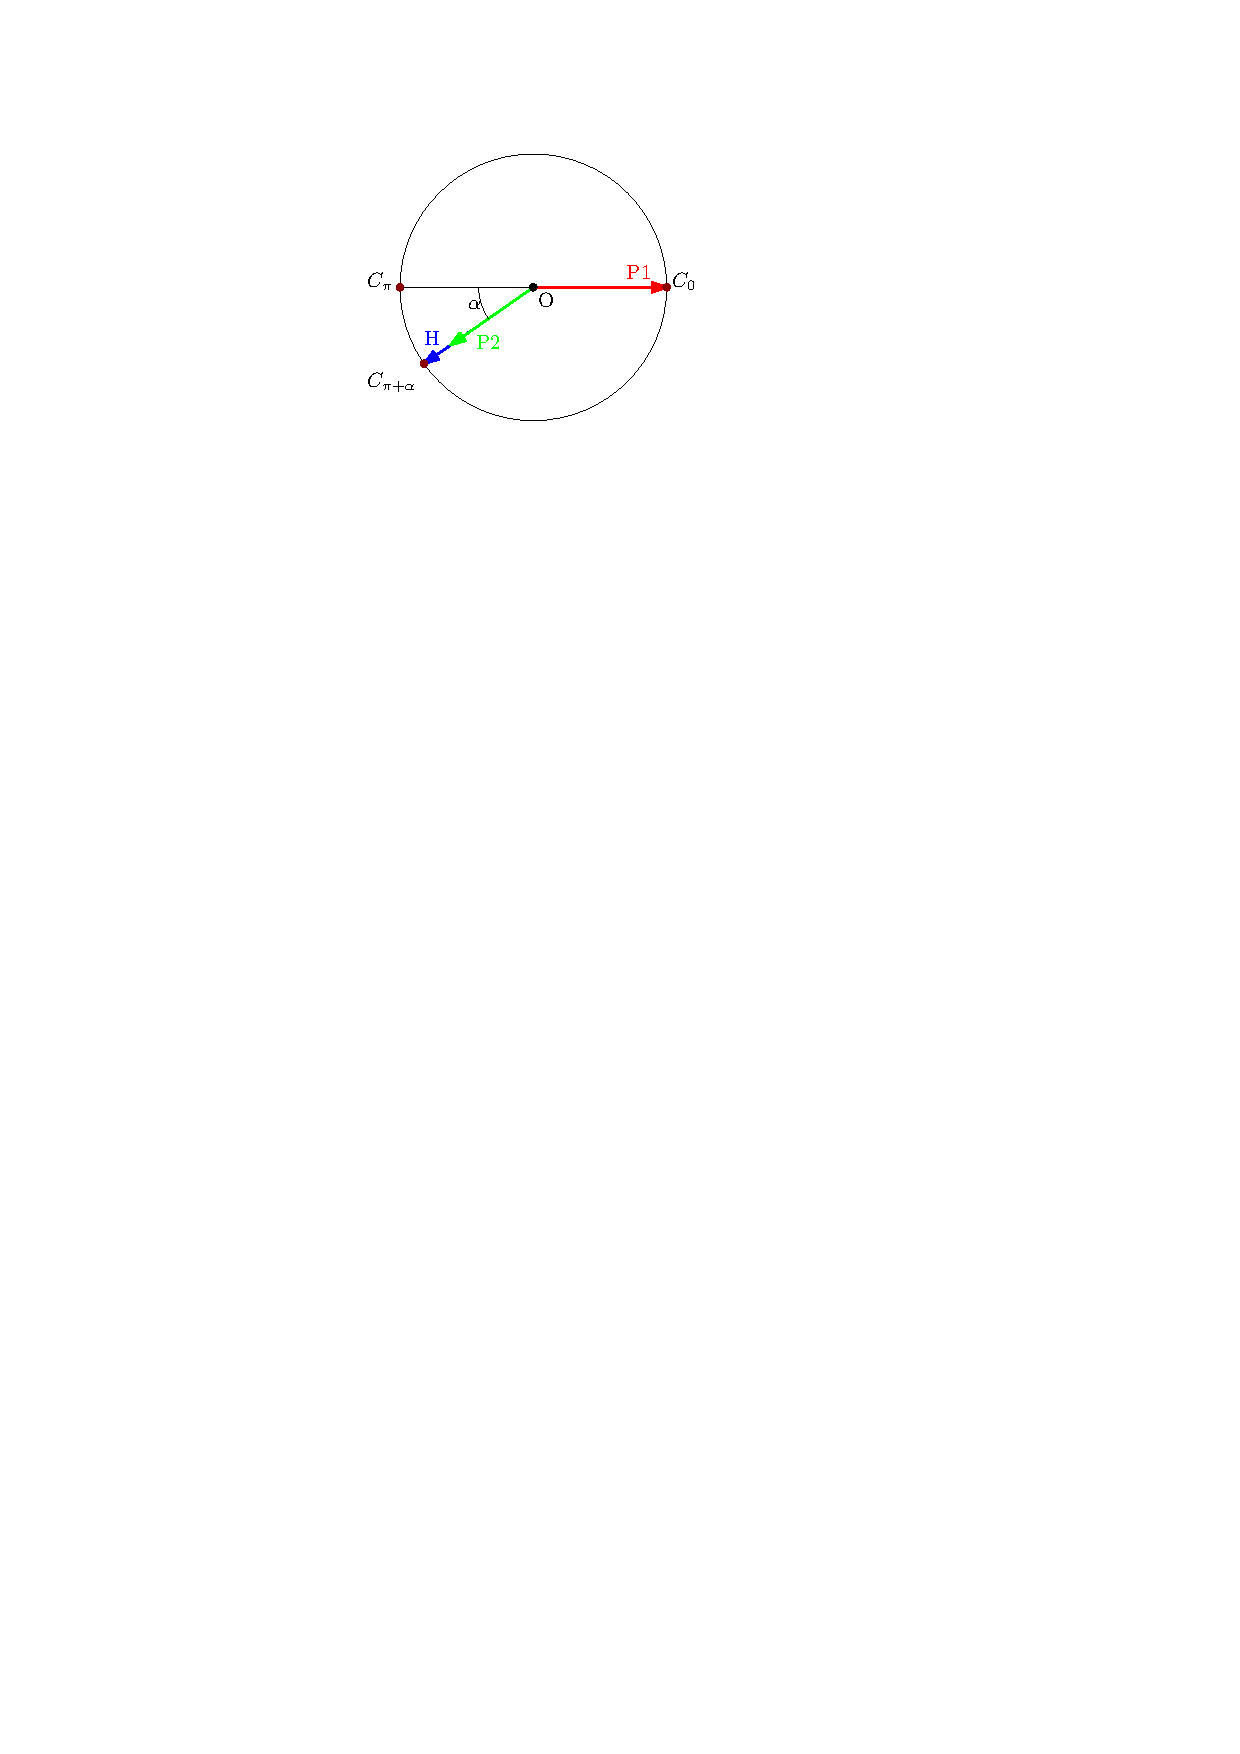
\includegraphics{mypics/2Q1S_references.pdf} \hfill
\end{center}

\begin{center}
    \textbf{Figure 1}: Reference points.
\end{center}

\begin{flushleft}

\vspace*{5mm} \textbf{Lemma 1}: The upper bound of the distance between two speed-1 agents converging on an unexplored arc
of a unit disk with angle $a >= 2\pi/3$ occurs when the agents are $\sqrt{3}$ away from
each other at the time of exit discovery.
\begin{center}
    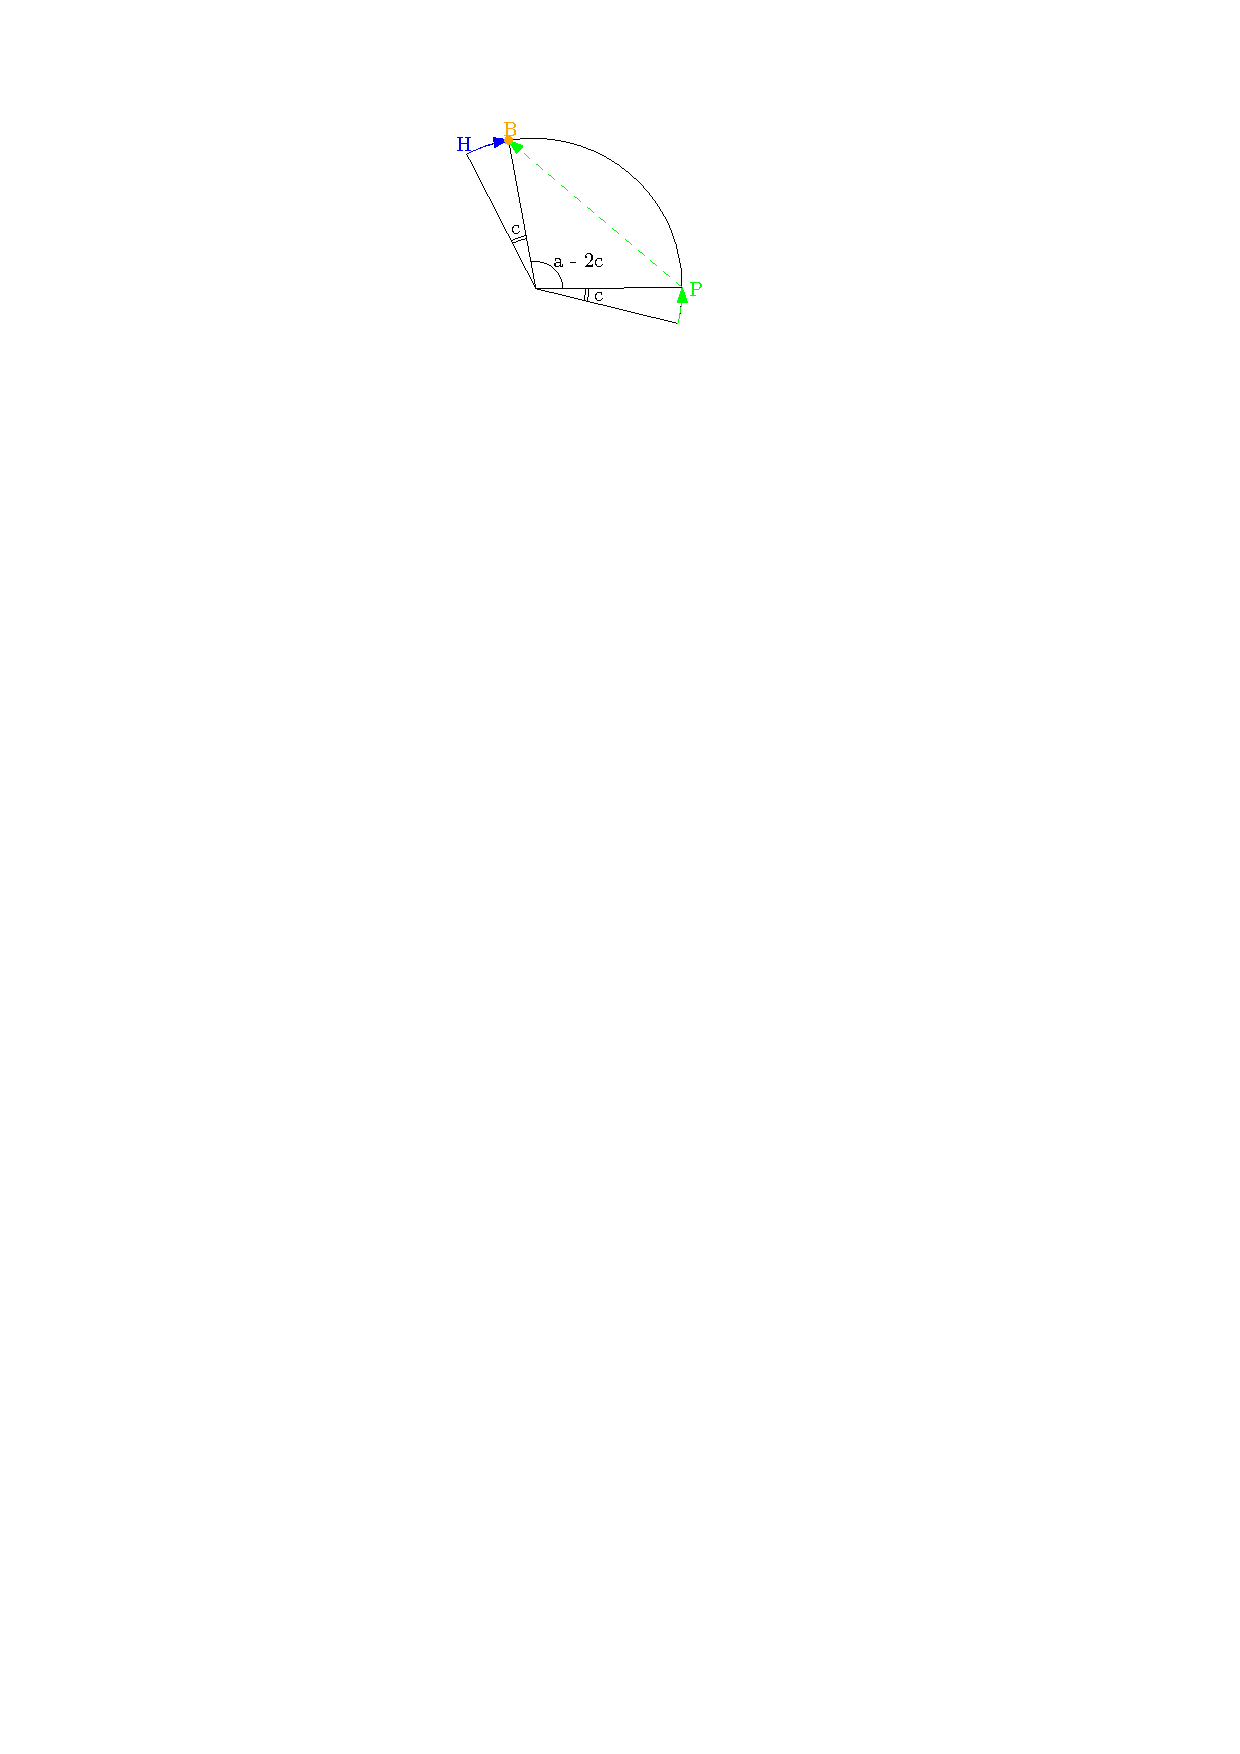
\includegraphics{mypics/lemma1-references.pdf}
\end{center}
\vspace*{5mm} \textbf{Proof}: Suppose the helper $H$ finds the exit at some point $B$ after the agents
have traveled a distance of $c$ along the arc. Then, the total time taken by the priority agent P
to get to $B$, having started at the opposite side of the arc $a$, would be:

\[ t = c + 2 \sin (\frac{a - 2c}{2}) \]

\vspace*{5mm} Then, differentiating with respect to $t$, we get:

\[ \frac{dt}{dc} = 1 - 2 \cos (\frac{a - 2c}{2}) \]

\vspace*{5mm} Finally, setting that equal to zero results in:

\[ \frac{2\pi}{3} = a - 2c \]

\vspace*{5mm} Thus, the greatest value for $t$ will occur when the agents are $\sqrt{3}$ apart,
or at an angle of $ \frac{2\pi}{3}$ for $a >= \frac{2\pi}{3}$ at the time of exit discovery.

%%%%%%%%%%%%%%%%%%%%%%%%%%%%%%%%%%%%%%%%%%%%%%%%%%%%%%%%%%%%%%%%%%%%%%%%%%%%%%%%%%%%%%%
%Marks end of section 2 so that it doesnt make the title of section 3 on the same page%
%If there are issues remove it                                                        %
%%%%%%%%%%%%%%%%%%%%%%%%%%%%%%%%%%%%%%%%%%%%%%%%%%%%%%%%%%%%%%%%%%%%%%%%%%%%%%%%%%%%%%%
\vfill

\end{flushleft}

\section{Algorithm Using a Detour}

\subsection{Evacuation Algorithm $Search_{2}$}

% Our second algorithm with 2 queens and 1 servant.
\begin{center}
    \begin{tabular}{ | p{1.5cm} || r l | l |}
        \hline
        \multicolumn{4} { | c | }{ Algorithm \textbf{$Search_{2}$}($\alpha$, $c$, $h$)} \\ \hline
        \textbf{Robot} & $\textbf{\#}$ & \textbf{Trajectory} & \textbf{Exit Protocol} \\ \hline
        \multirow{2}{*}{$P1$} & 0 & Travel from $O$ to $C_{0}$. & IF: Exit found by $P1$ - Done. \\
        & 1 & Travel CCW for $c$ time. & ELSE: Travel along chord to exit if closer. \\
        & 2 & Travel directly to $C_{c+h}$. & \\
        & 3 & Travel CW. & \\ \hline
        \multirow{2}{*}{$P2$} & 0 & Travel from $O$ to $C_{\pi + \alpha}$ & IF: Exit found by $P2$ - Done. \\
        & 1 & Travel CCW. & ELSE: Travel along a chord to exit if closer.\\ \hline
        \multirow{2}{*}{$H$} & 0 & Travel from $O$ to $C_{\pi + \alpha}$ & \multirow{2}{*}{Broadcast exit location and then wait.} \\
        & 1 & Travel CW. & \\ \hline
    \end{tabular}
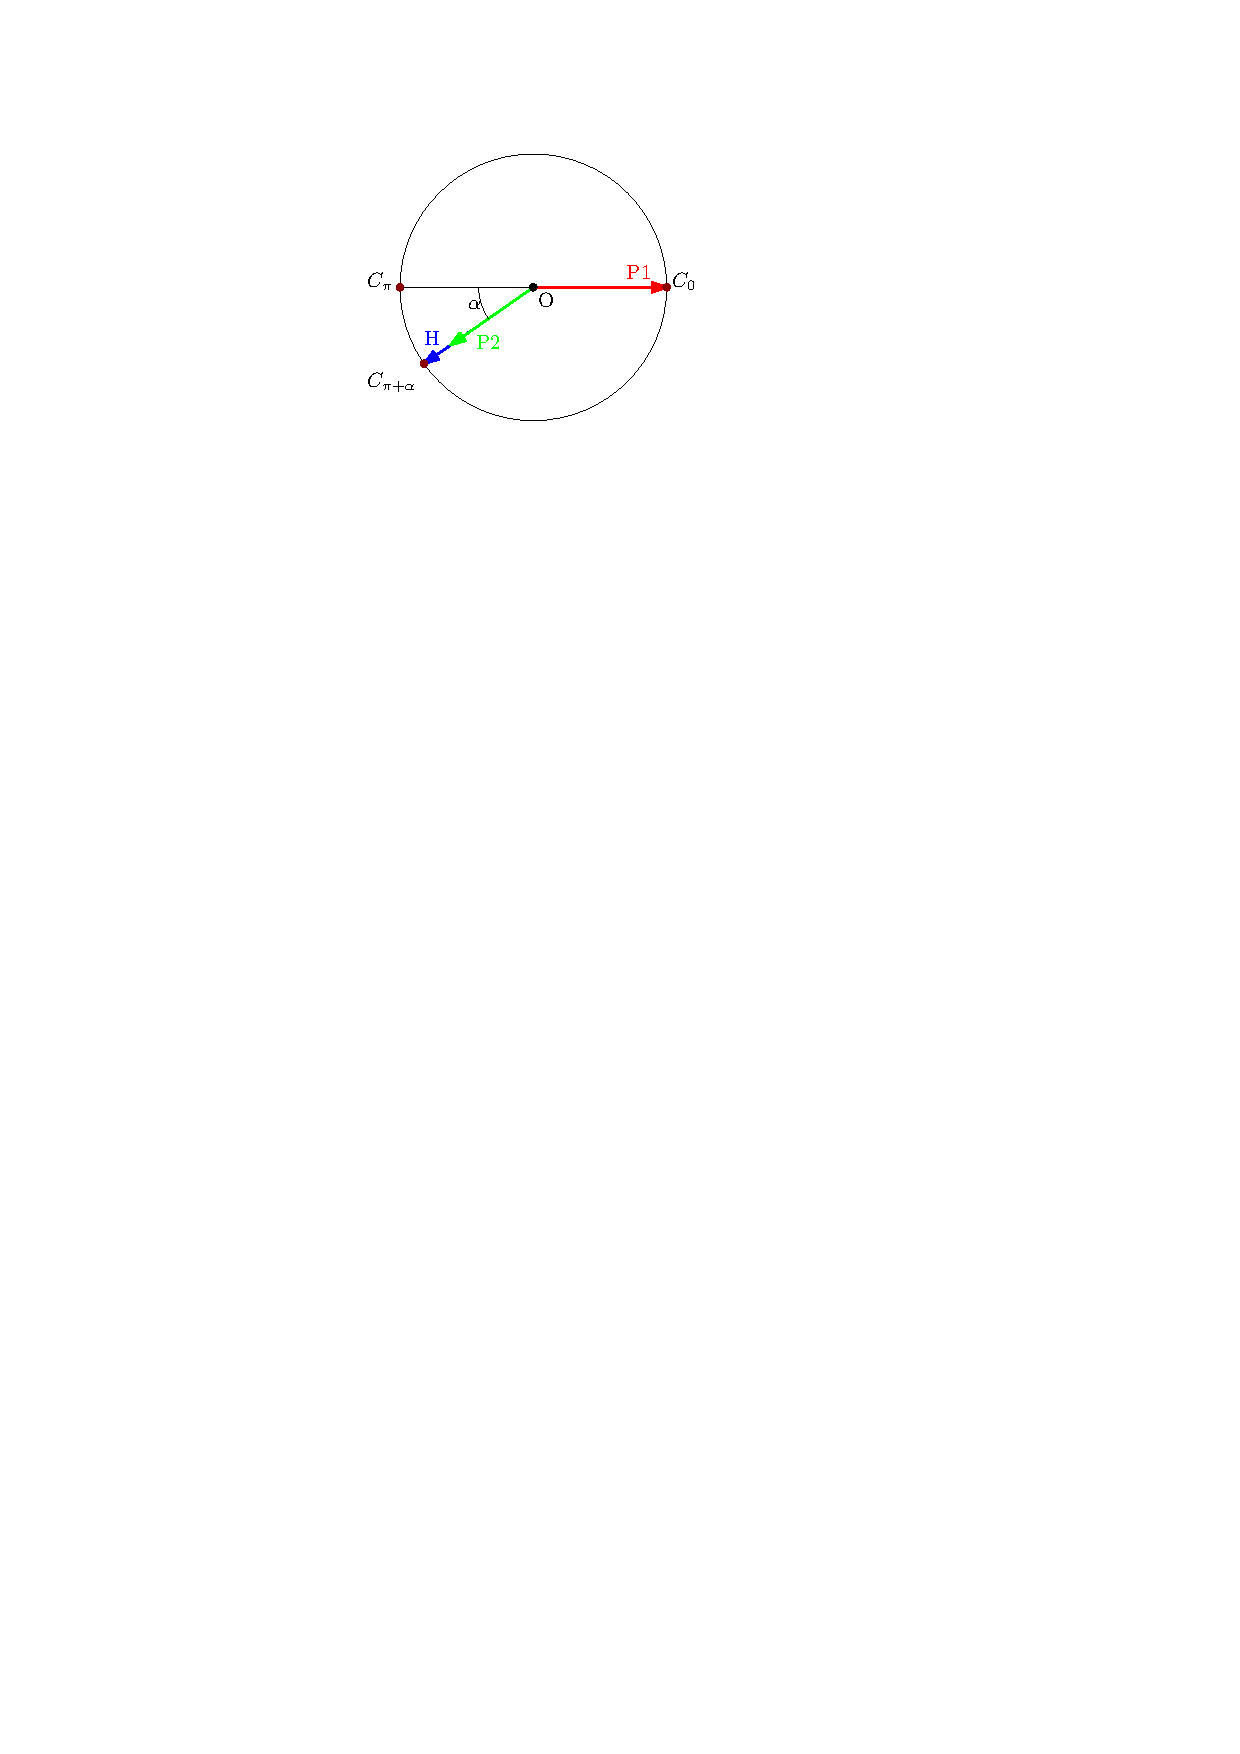
\includegraphics{mypics/2Q1S_references.pdf} \hfill
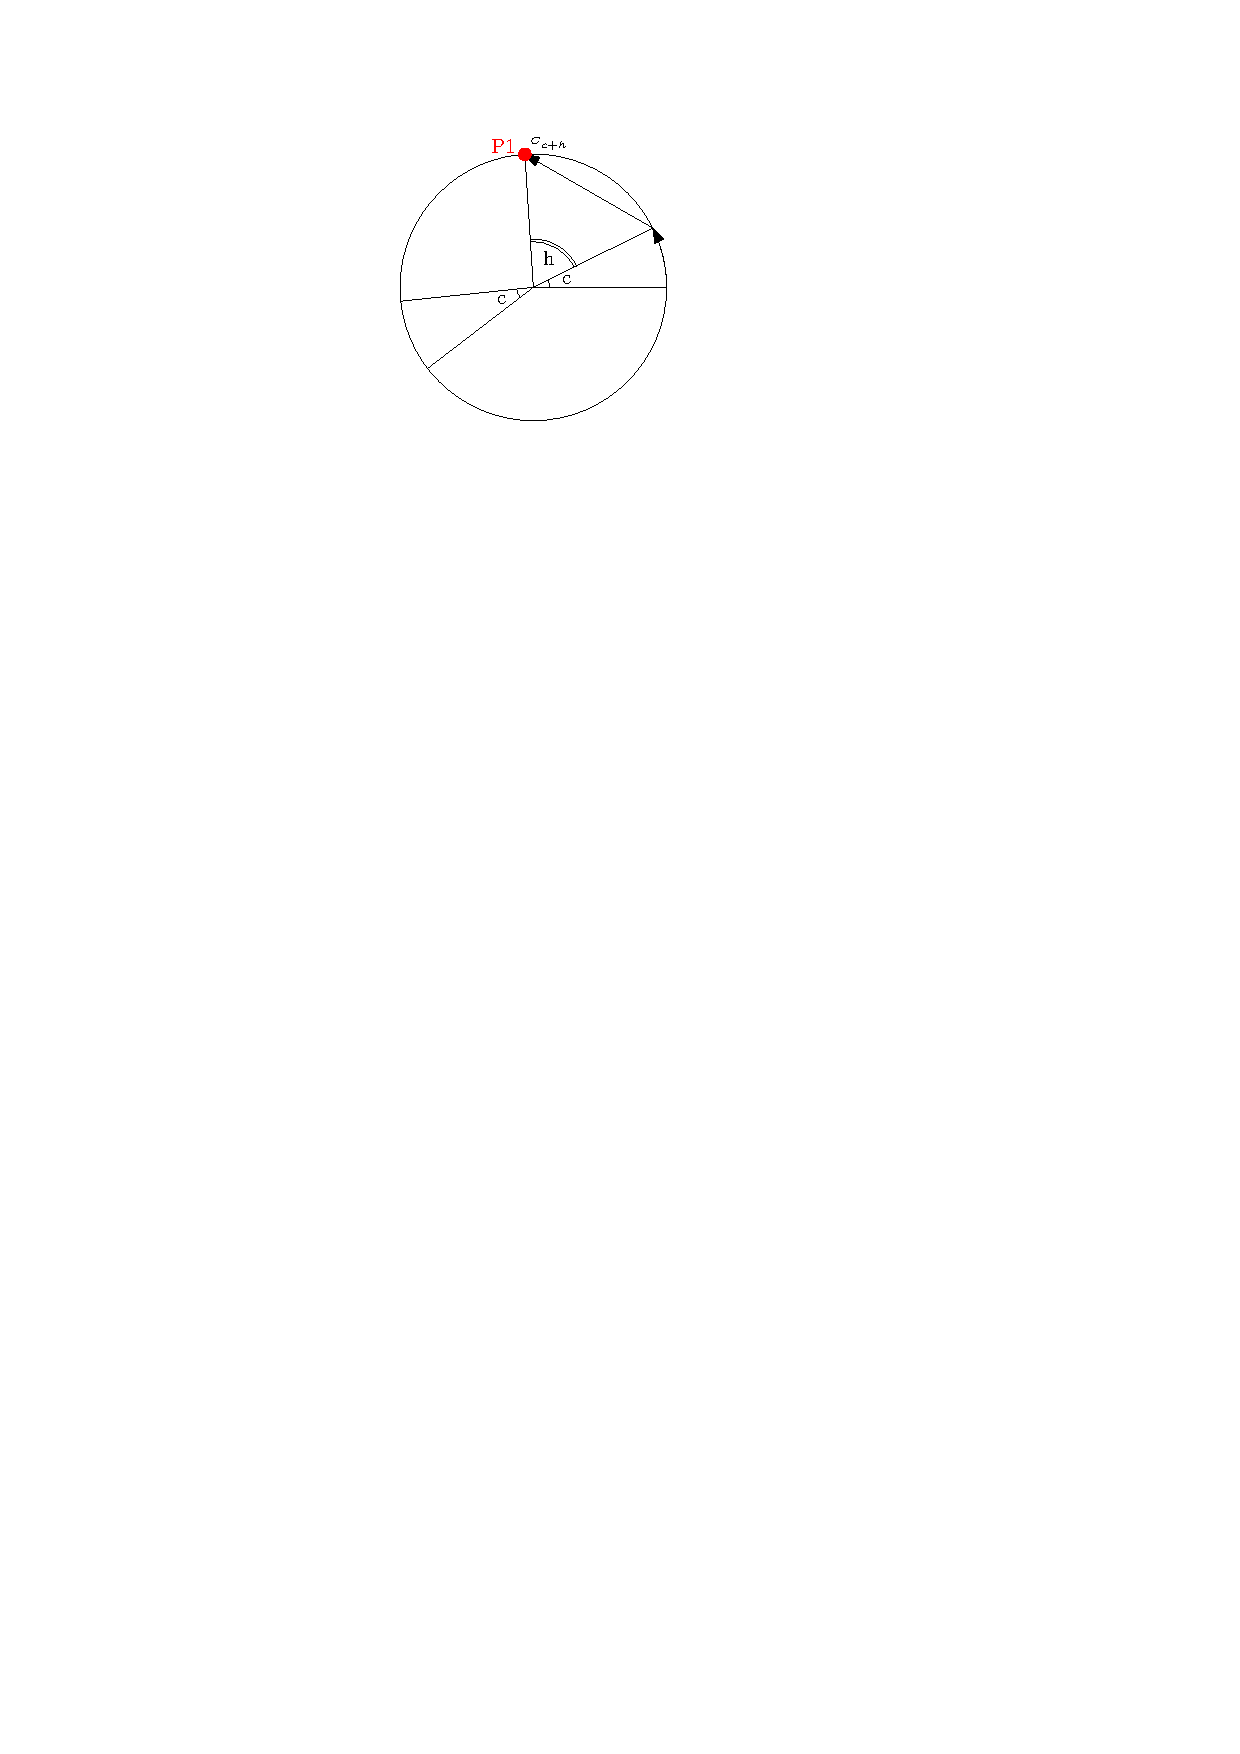
\includegraphics{Q2S1_Eq/Q2S1_DetourExample.pdf}
\end{center}
\begin{flushleft}
    In this algorithm, $P1$ utilizes a detour, abandoning its search along the wall
    in favor of getting closer to $H$ in anticipation of the exit being found when both
    priority are equidistant from $H$ at the time of exit discovery. By doing this, we minimize
    $P2$'s responsibility to $H$ allowing it to search the bottom wall faster. Then, by
    \textbf{Lemma 1} we can prove that for a certain value $c$ and $h$, the total time until $P1$
    evacuates is decreasing until the end of its detour, and constant for the rest of its seach, as
    it will always be a constant distance $h$ away from the Helper during its last phase.
\end{flushleft}

\subsection{Equations}

\begin{flushleft}
    First, we know that we can divide the circle into two sections, where $a$ is the
    responsibility of the $H$ and $P1$, and the $b$ is the responsibility of $P2$.
    Therefore:

    \begin{tabularx}{\textwidth}{lXc}
        \multirow{2}{*}{$2\pi = a+b$} & & \parbox[c]{0.25\textwidth}{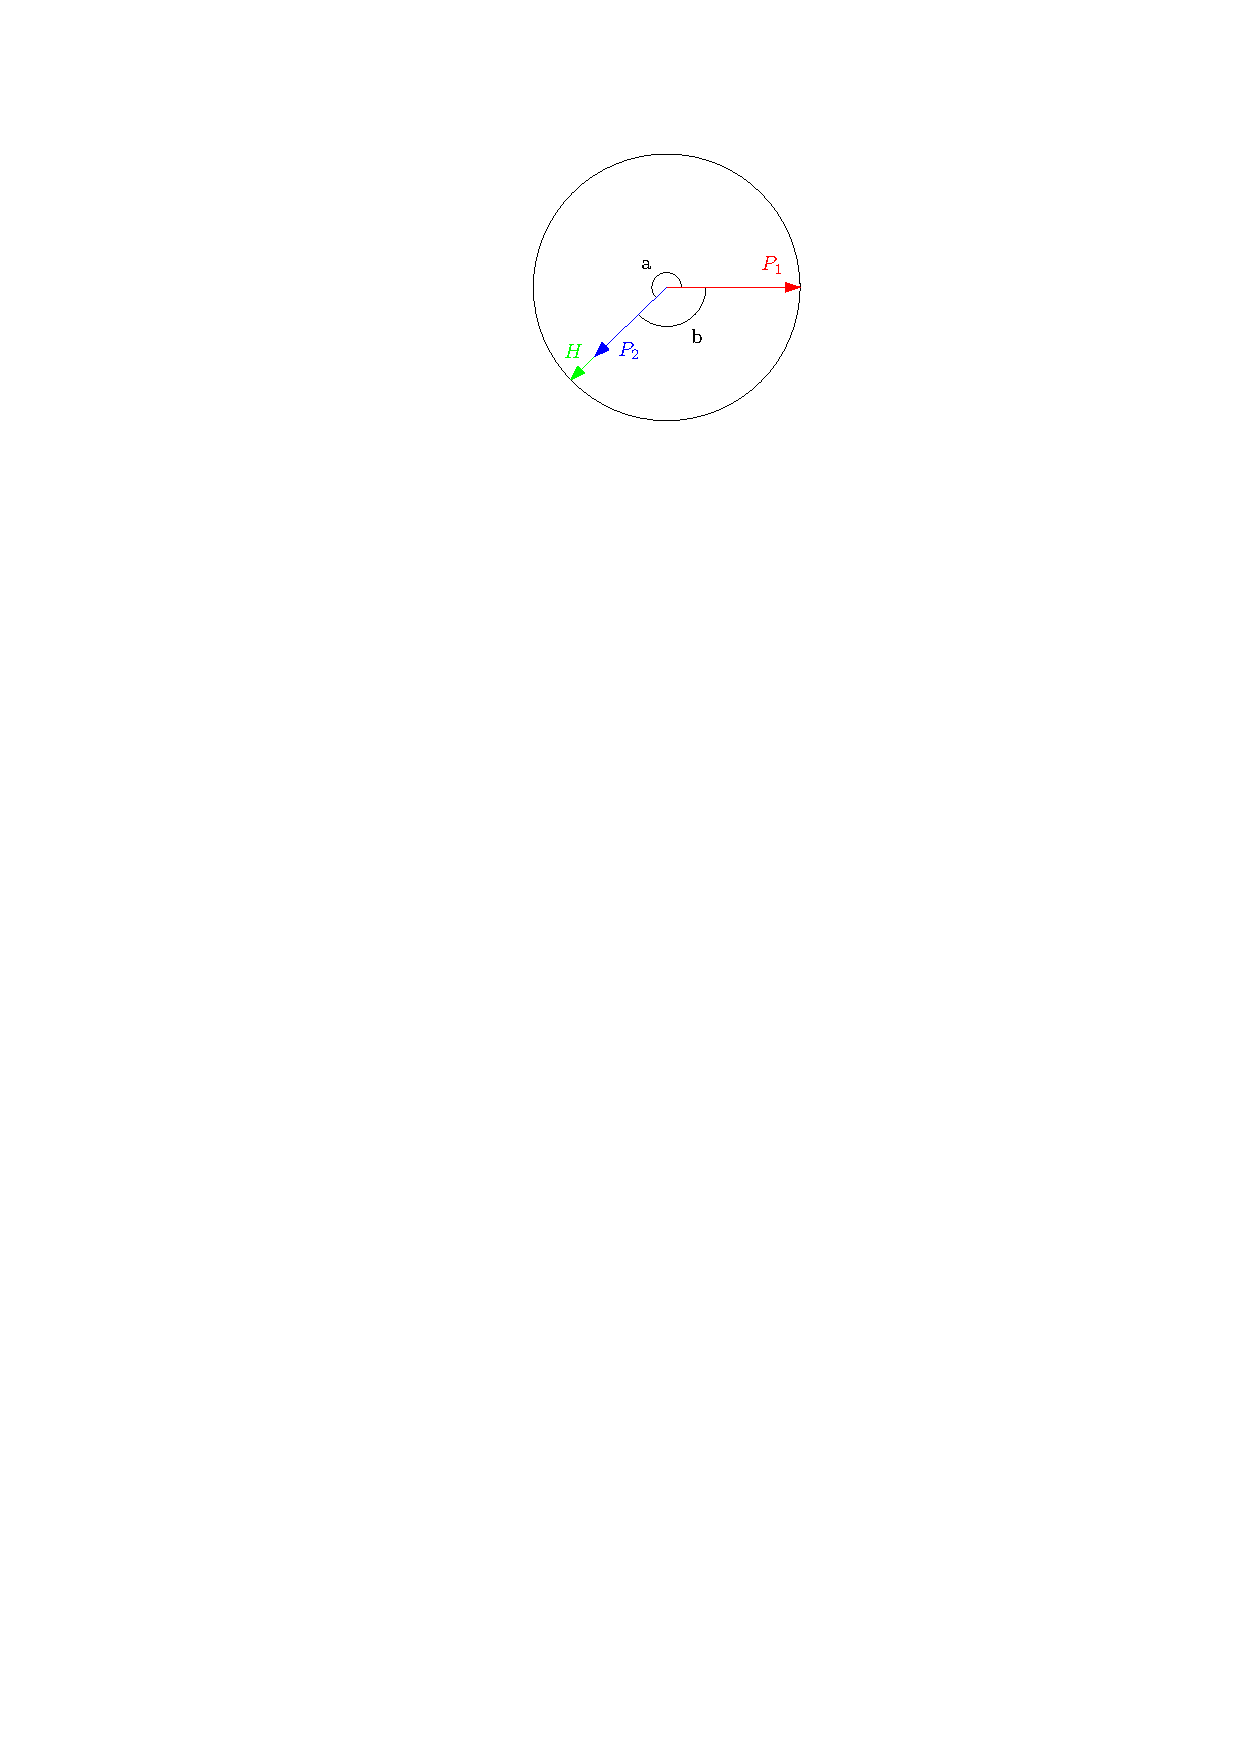
\includegraphics[width=0.25\textwidth]{Q2S1_Eq/eq_1.pdf}} \\
    \end{tabularx}

    We know that $P1$ and $H$ will have to travel a total of $a$ around the circle,
    and after a certain time $c$, the remaining unsearched area will be

    \begin{tabularx}{\textwidth}{lXc}
        \multirow{2}{*}{$a = 2c+d$} & & \parbox[c]{0.25\textwidth}{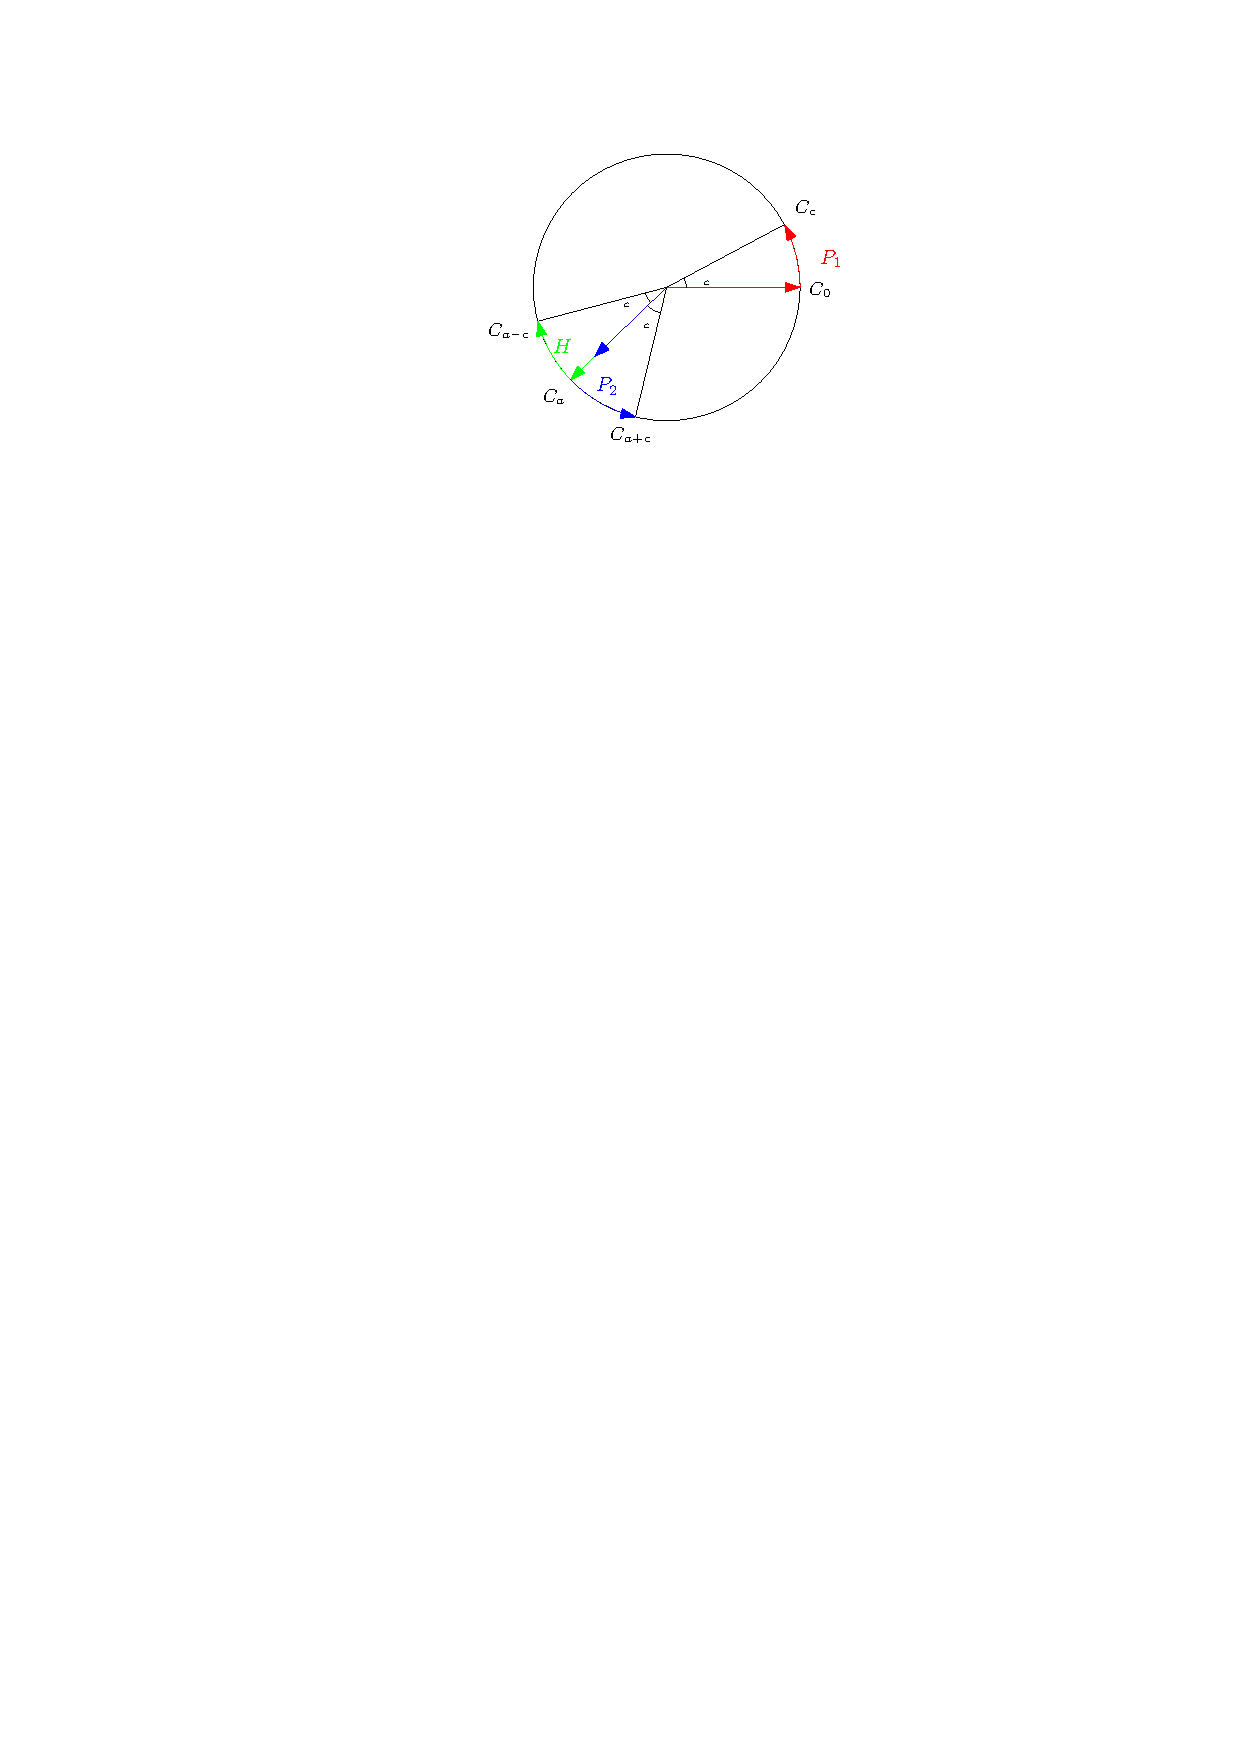
\includegraphics[width=0.25\textwidth]{Q2S1_Eq/eq_2.pdf}} \\
    \end{tabularx}




    If, after more time $e$ of both agents following the perimeter the distance between the two
    would be equal to $\sqrt{3}$, which by Lemma 1 will result in the evacuation time increasing, then
    we instead send $P1$ along a chord of angle $h$, such that when $H$ reaches point $C_{a - c - e}$, $P1$ will be travelling somewhere along the chord.

    \begin{tabularx}{\textwidth}{lXc}
        \multirow{2}{*}{$c+e = \frac{a - \frac{2\pi}{3}}{2}$} & &  \parbox[c]{0.25\textwidth}{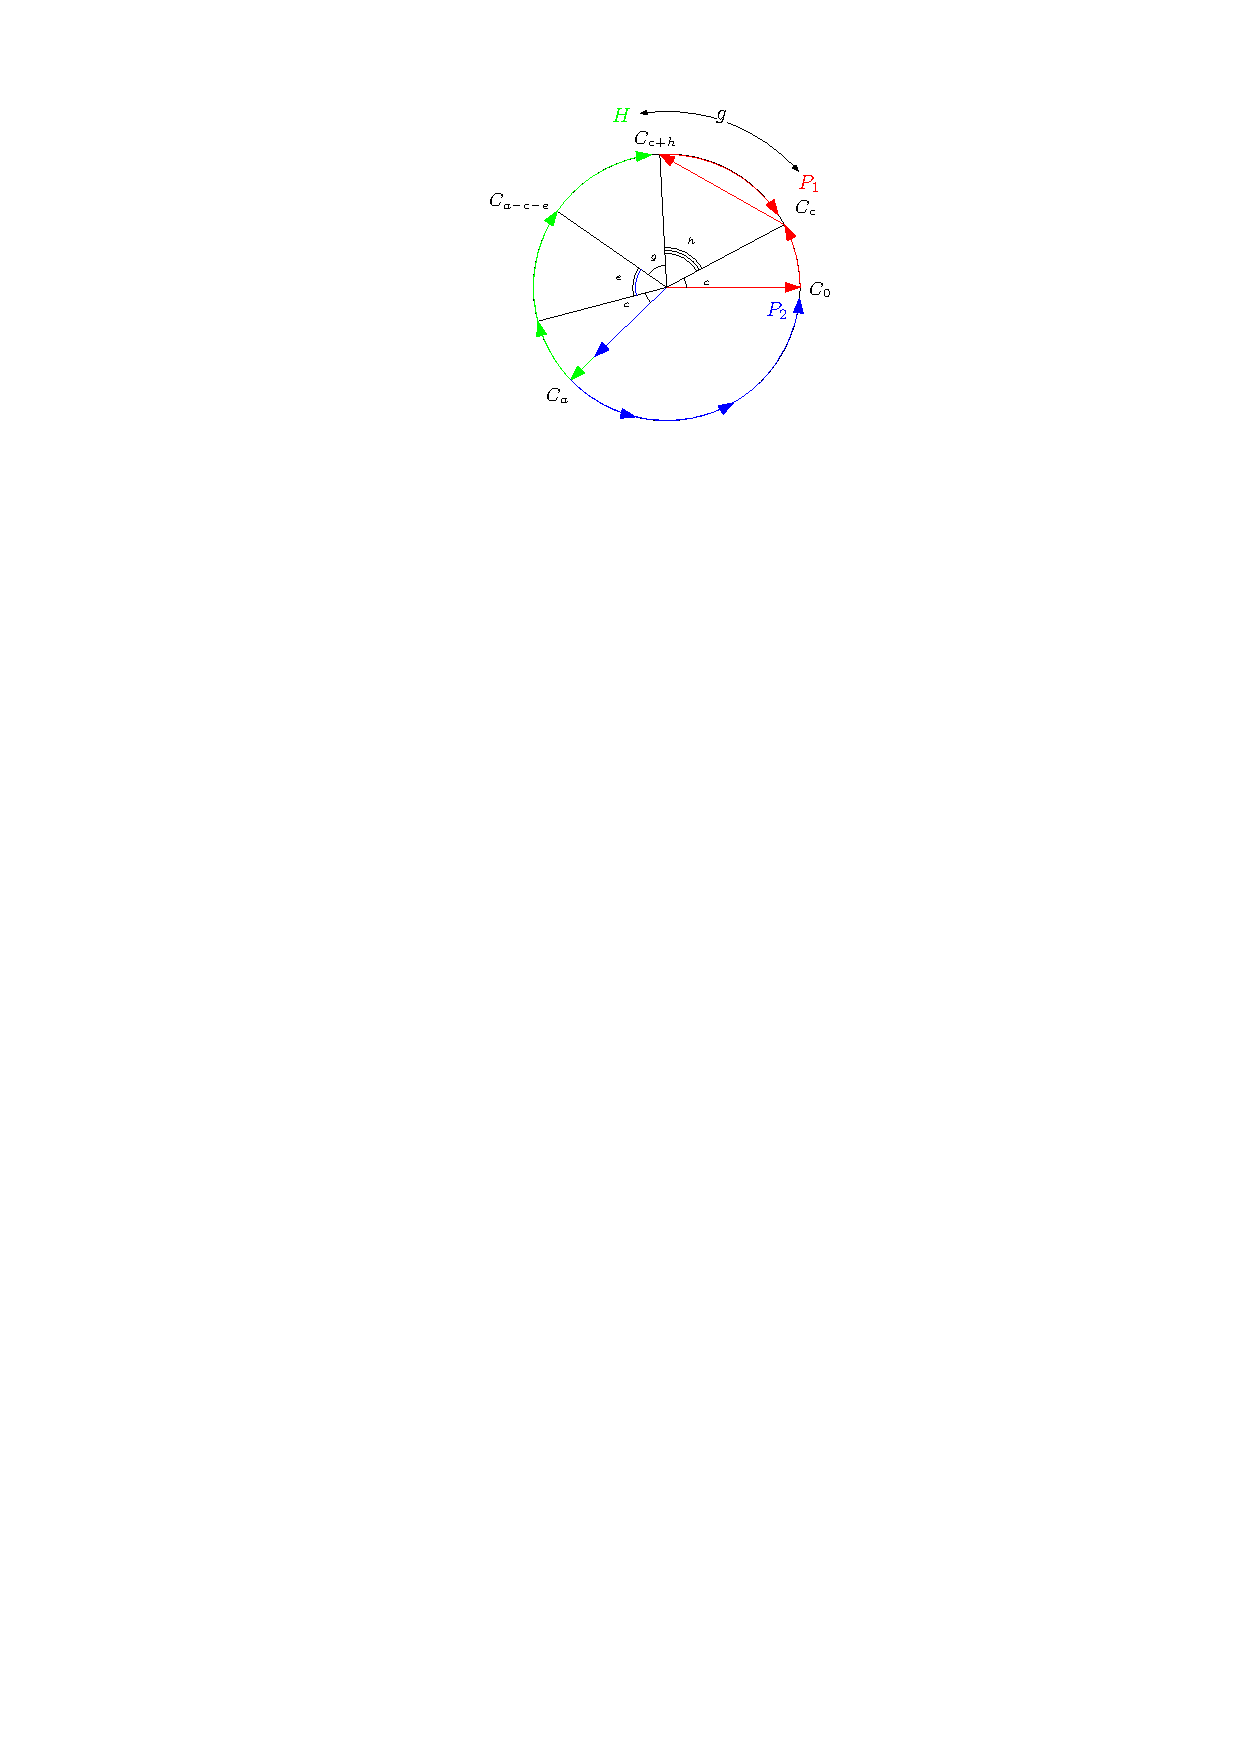
\includegraphics[width=0.25\textwidth]{Q2S1_Eq/eq_4.pdf}} \\
    \end{tabularx}

    The point at which $P1$ reaches the end of the detour at point $C_{c + h}$,
    the $H$ will be at point $C_{a - c - e - f}$, where $f$ is the extra time
    taken by $P1$ to reach the end of its detour.

    \begin{tabularx}{\textwidth}{lXc}
        \multirow{2}{*}{$e+f = 2\sin(\frac{h}{2})$} & & \parbox[c]{0.3\textwidth}{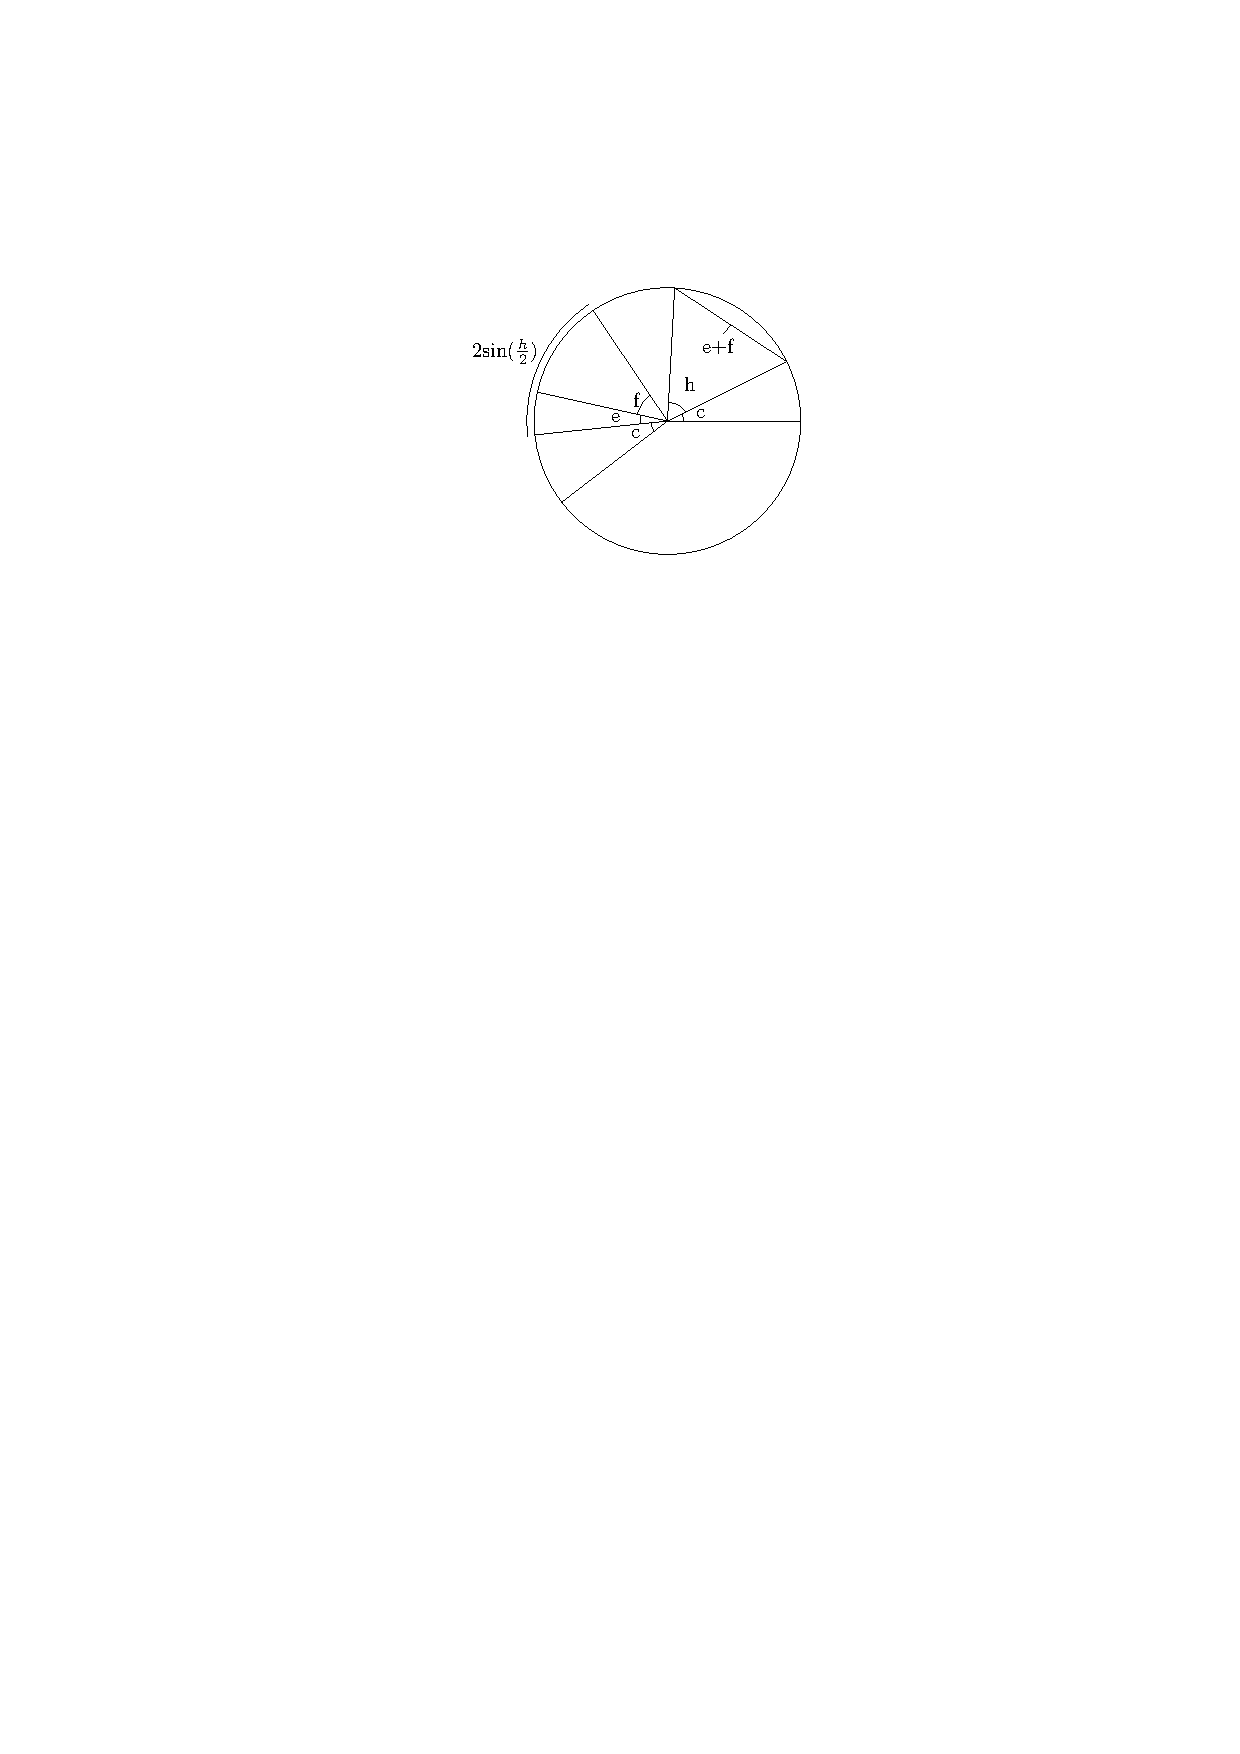
\includegraphics[width=0.3\textwidth]{Q2S1_Eq/eq_5.pdf}} \\
    \end{tabularx}

    We call $g$ the remaining unsearched arc between $C_{c + h}$ and $C_{a - c - e - f}$
    such that:

    \begin{tabularx}{\textwidth}{lXc}
        \multirow{2}{*}{$d = e+f+g+h$} & & \parbox[c]{0.25\textwidth}{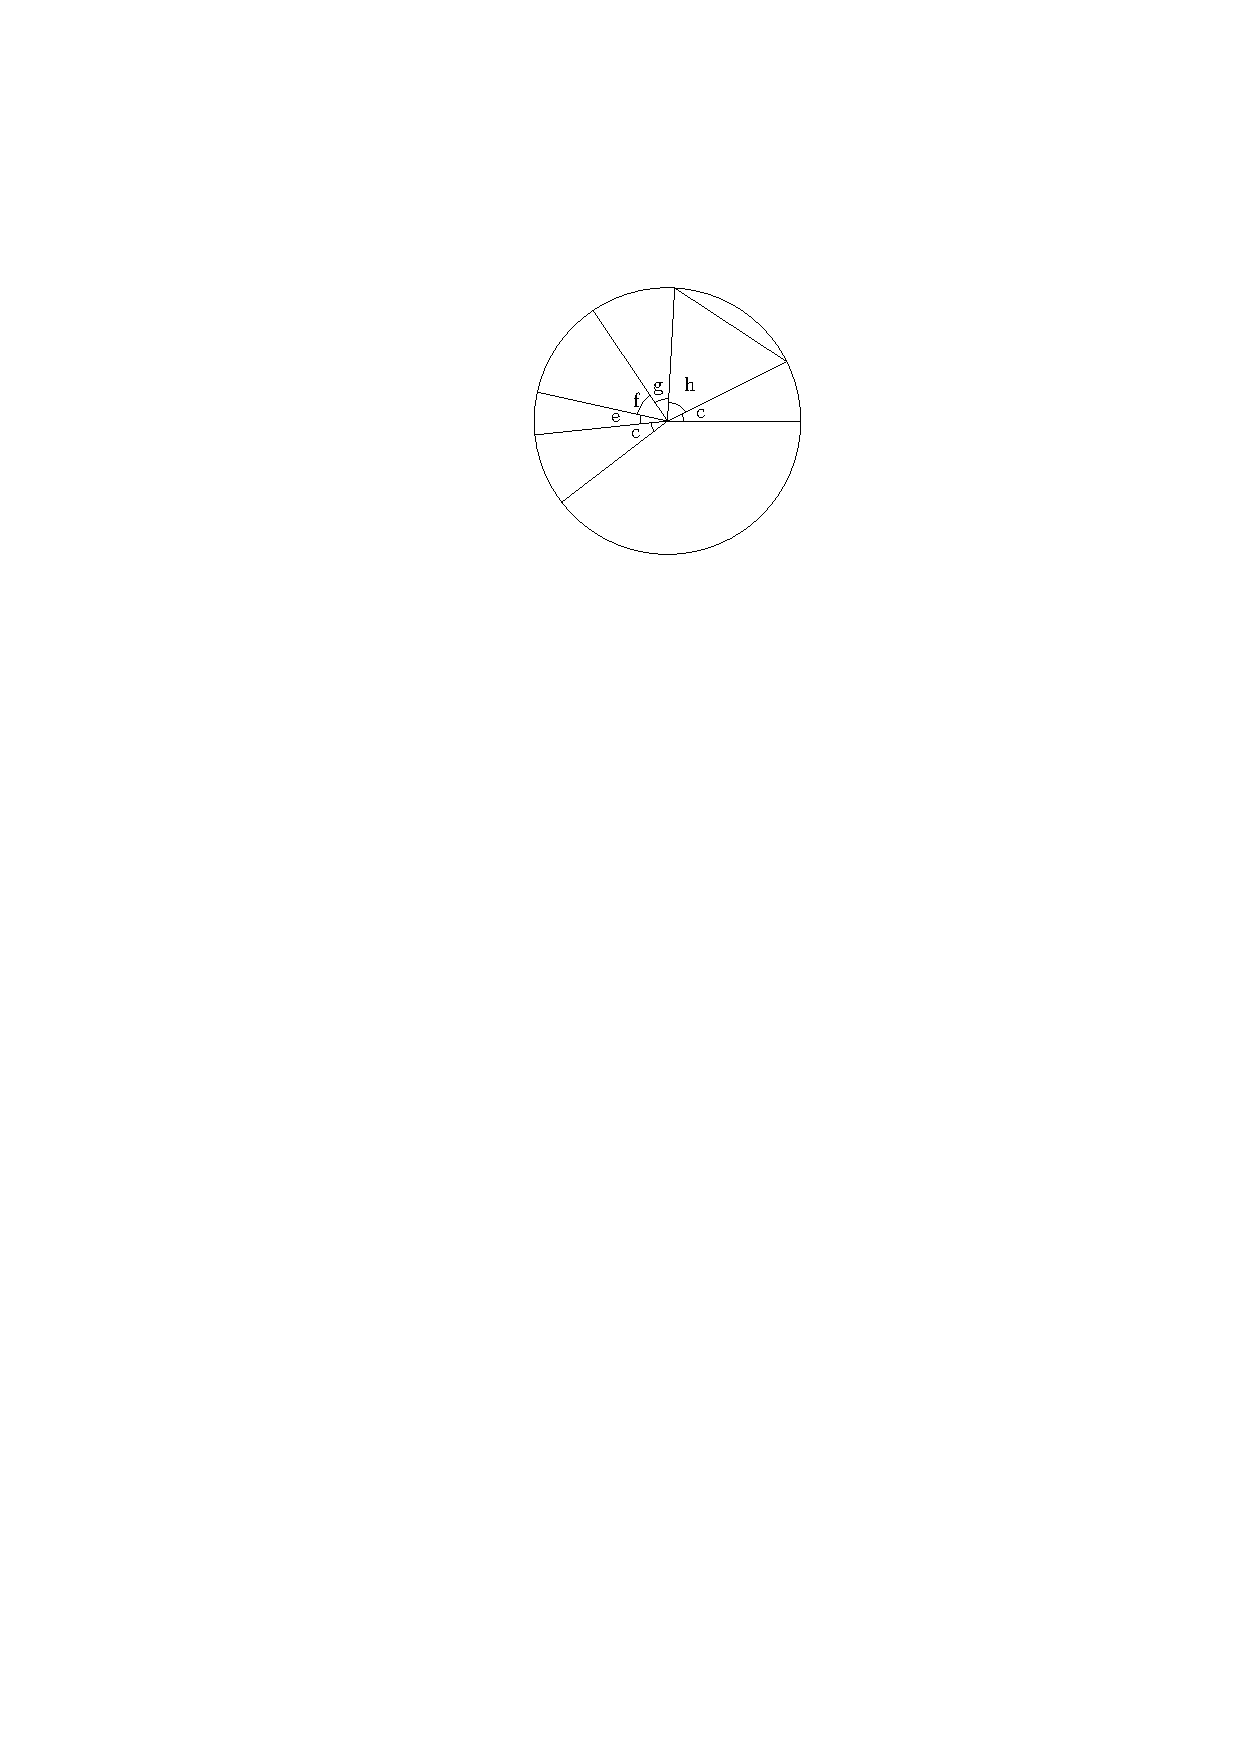
\includegraphics[width=0.25\textwidth]{Q2S1_Eq/eq_3.pdf}} \\
    \end{tabularx}

    At this point in the algorithm, we send $P1$ clockwise to search the area from $C_{c + h}$ until
    $C_{c}$ and $H$ stays clockwise to search the remaining area from $C_{a - c - e - f}$ until $C_{c + h}$. At this point the distance between the two agents stays constant for the rest of the algorithm, and this distance is equal to $2\sin(\frac{g}{2})$. Clearly, the optimal value for $h$ is:

    \begin{tabularx}{\textwidth}{lXc}
        \multirow{2}{*}{$h = g+2\sin(\frac{g}{2})$} & & \parbox[c]{0.25\textwidth}{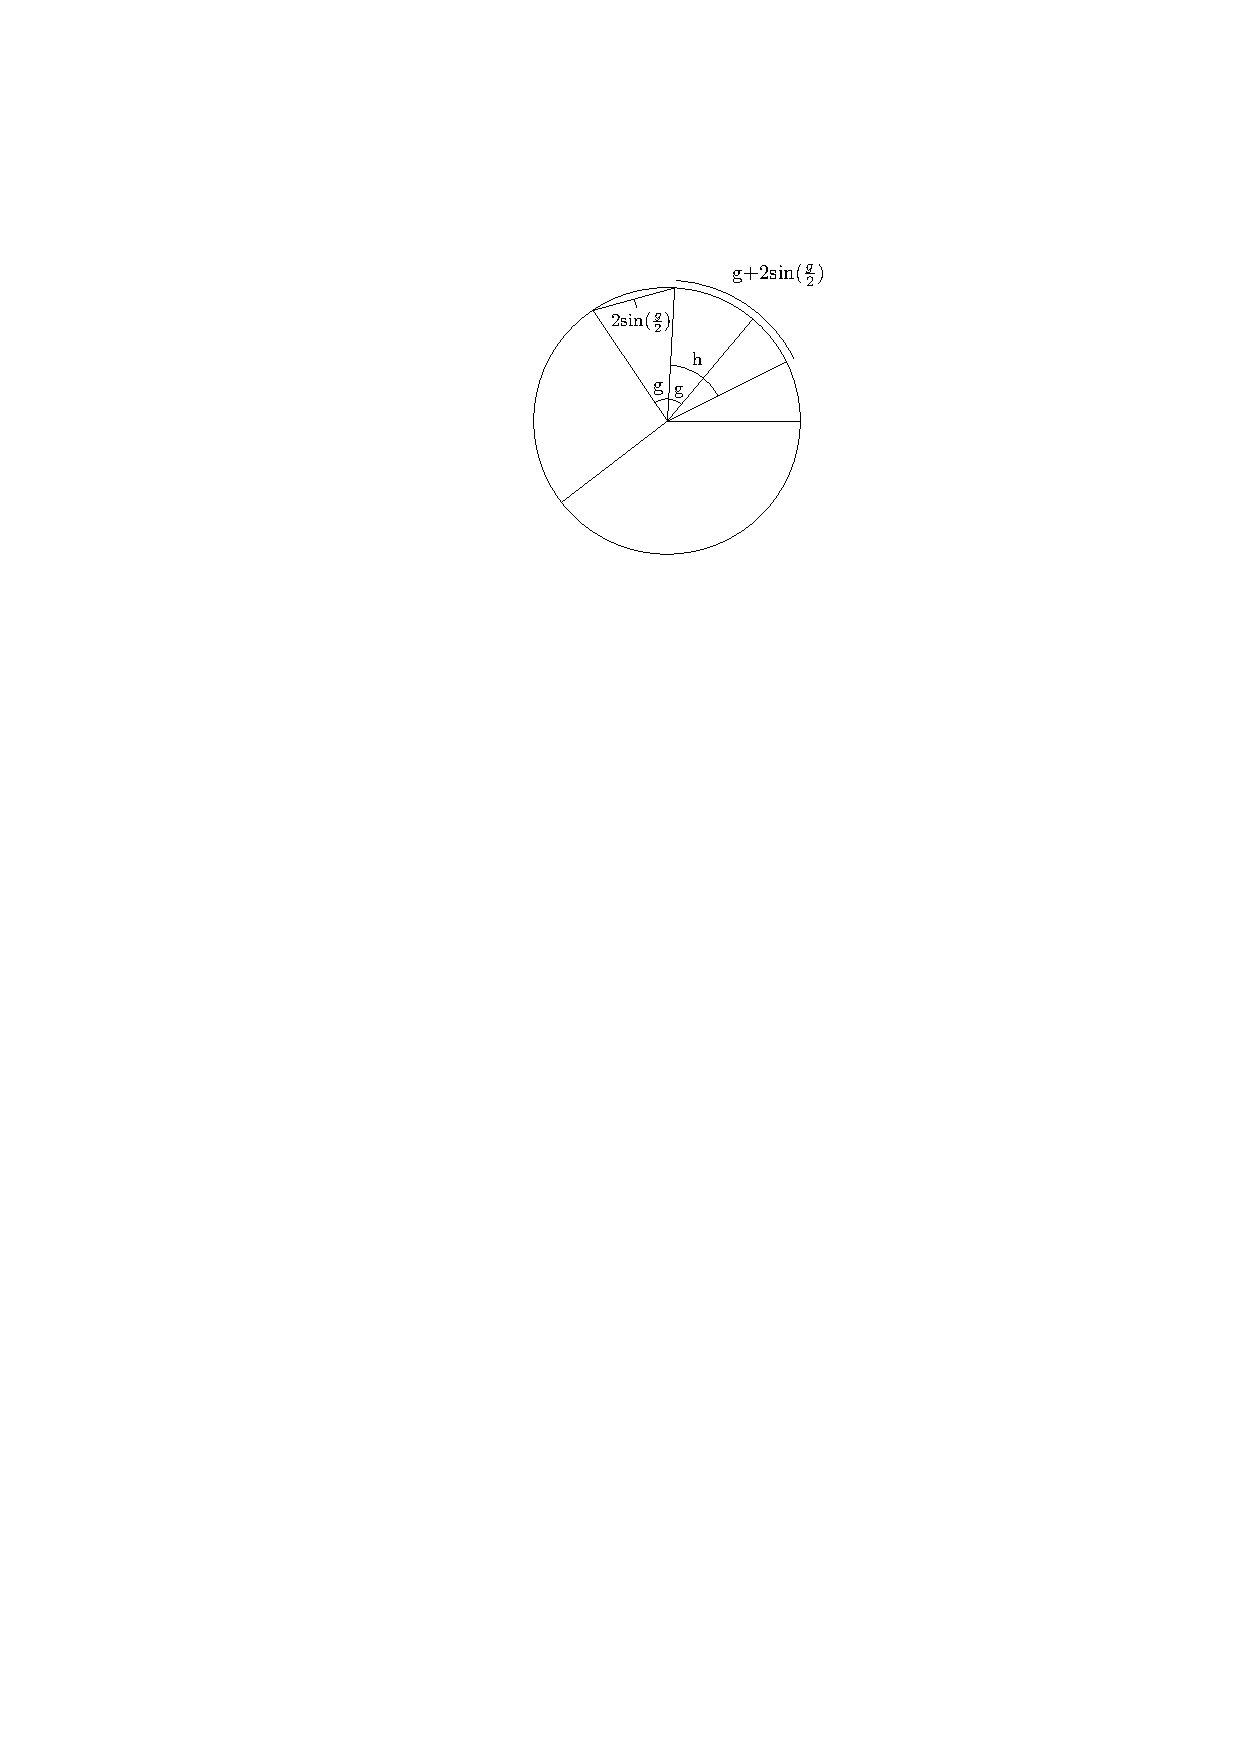
\includegraphics[width=0.25\textwidth]{Q2S1_Eq/eq_6.pdf}} \\
    \end{tabularx}


    At this point, we have fully partitioned the circle such that:

    \[ 2\pi = b + 2c + e + f + g + h\]

    which, once simplified, becomes:

    \[ 2\pi = b + 2c + 2\sin(\frac{g + 2\sin(\frac{g}{2})}{2}) + 2g + 2\sin(\frac{g}{2}) \]

    At this point, we identify three upper bounds. One is when $P2$ finds the exit at the end of its
    search, at

    \begin{tabularx}{\textwidth}{lXc}
        \multirow{2}{*}{$t = 1+b$} & & \parbox[c]{0.25\textwidth}{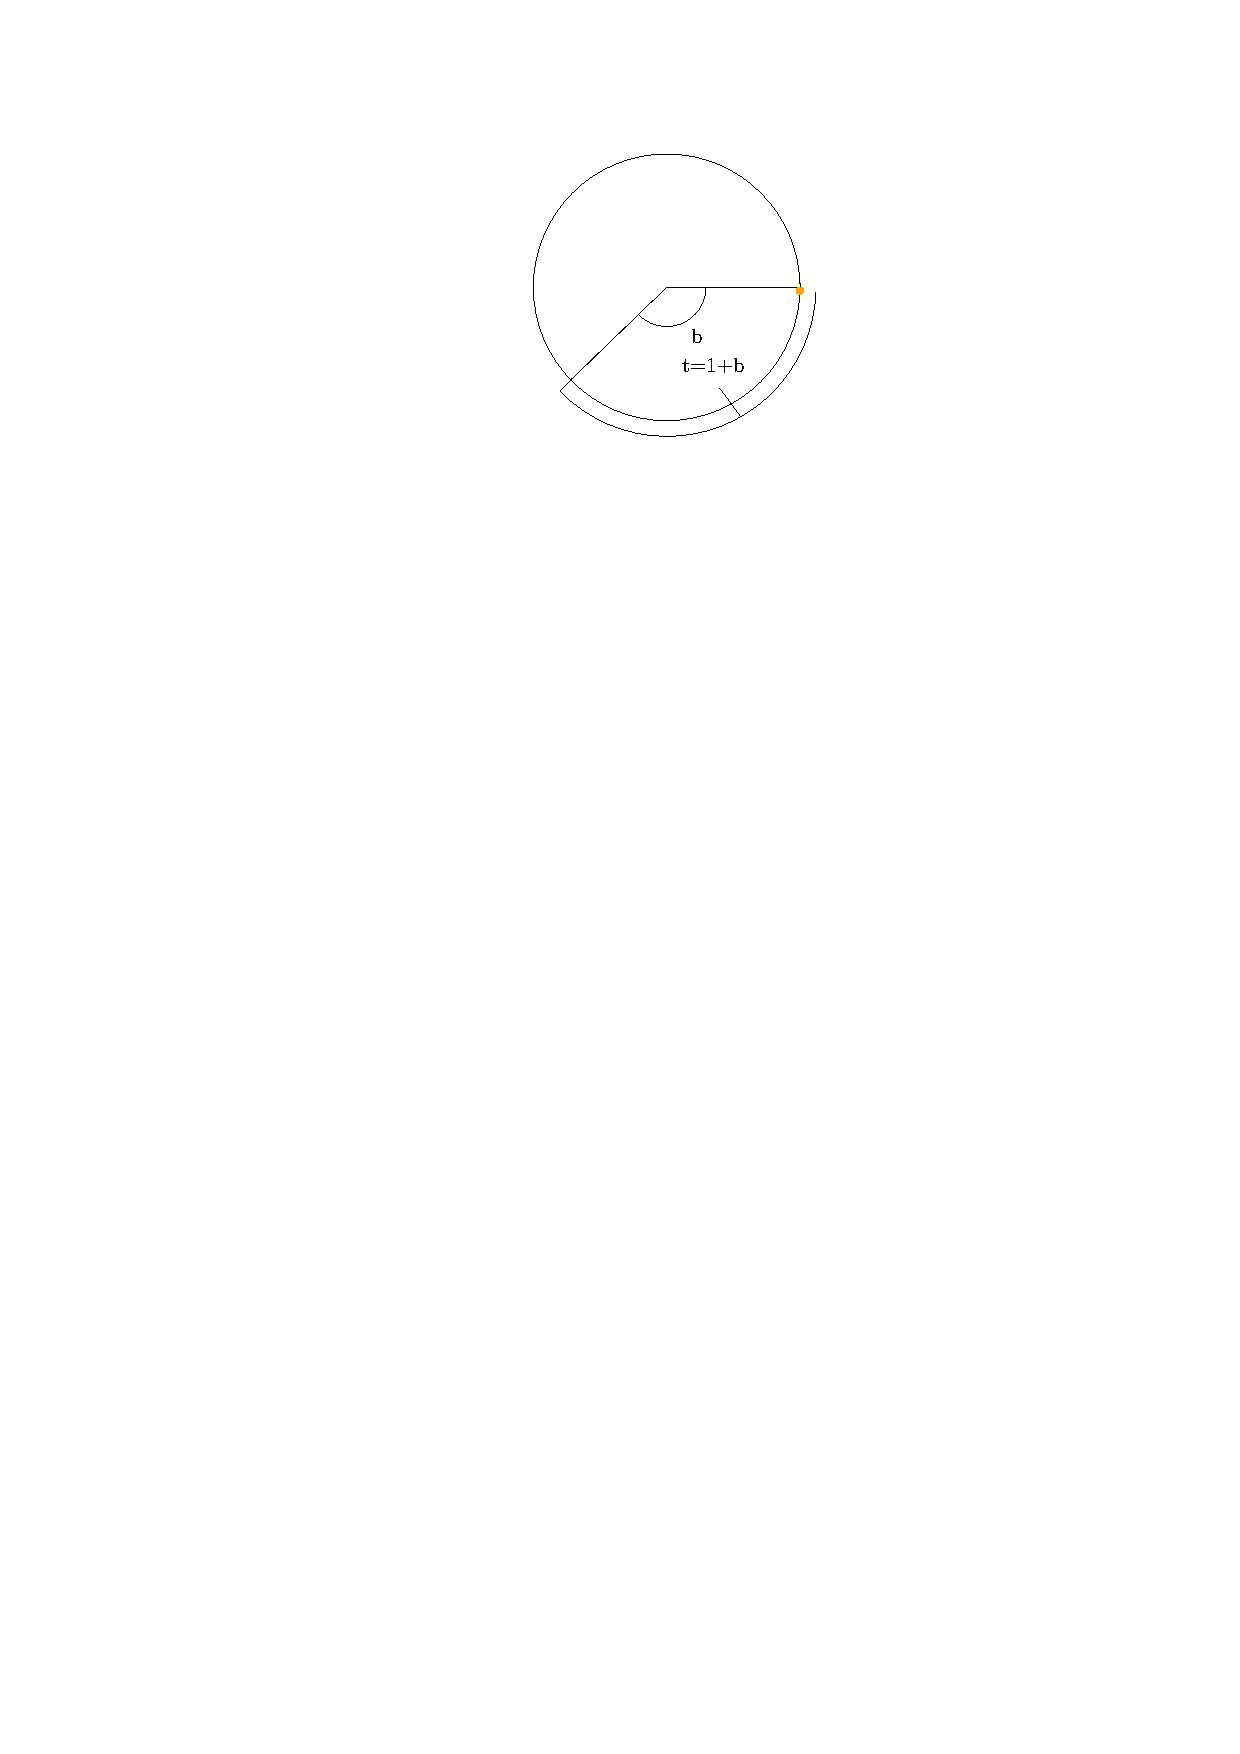
\includegraphics[width=0.25\textwidth]{Q2S1_Eq/ub_1.pdf}} \\
    \end{tabularx}

    Another upper bound occurs when either $H$ or $P1$ finds the exit at the end of
    their search, after time

    \begin{tabularx}{\textwidth}{lXc}
        \multirow{2}{*}{$t = 1+c+e+f+h$} & & \parbox[c]{0.25\textwidth}{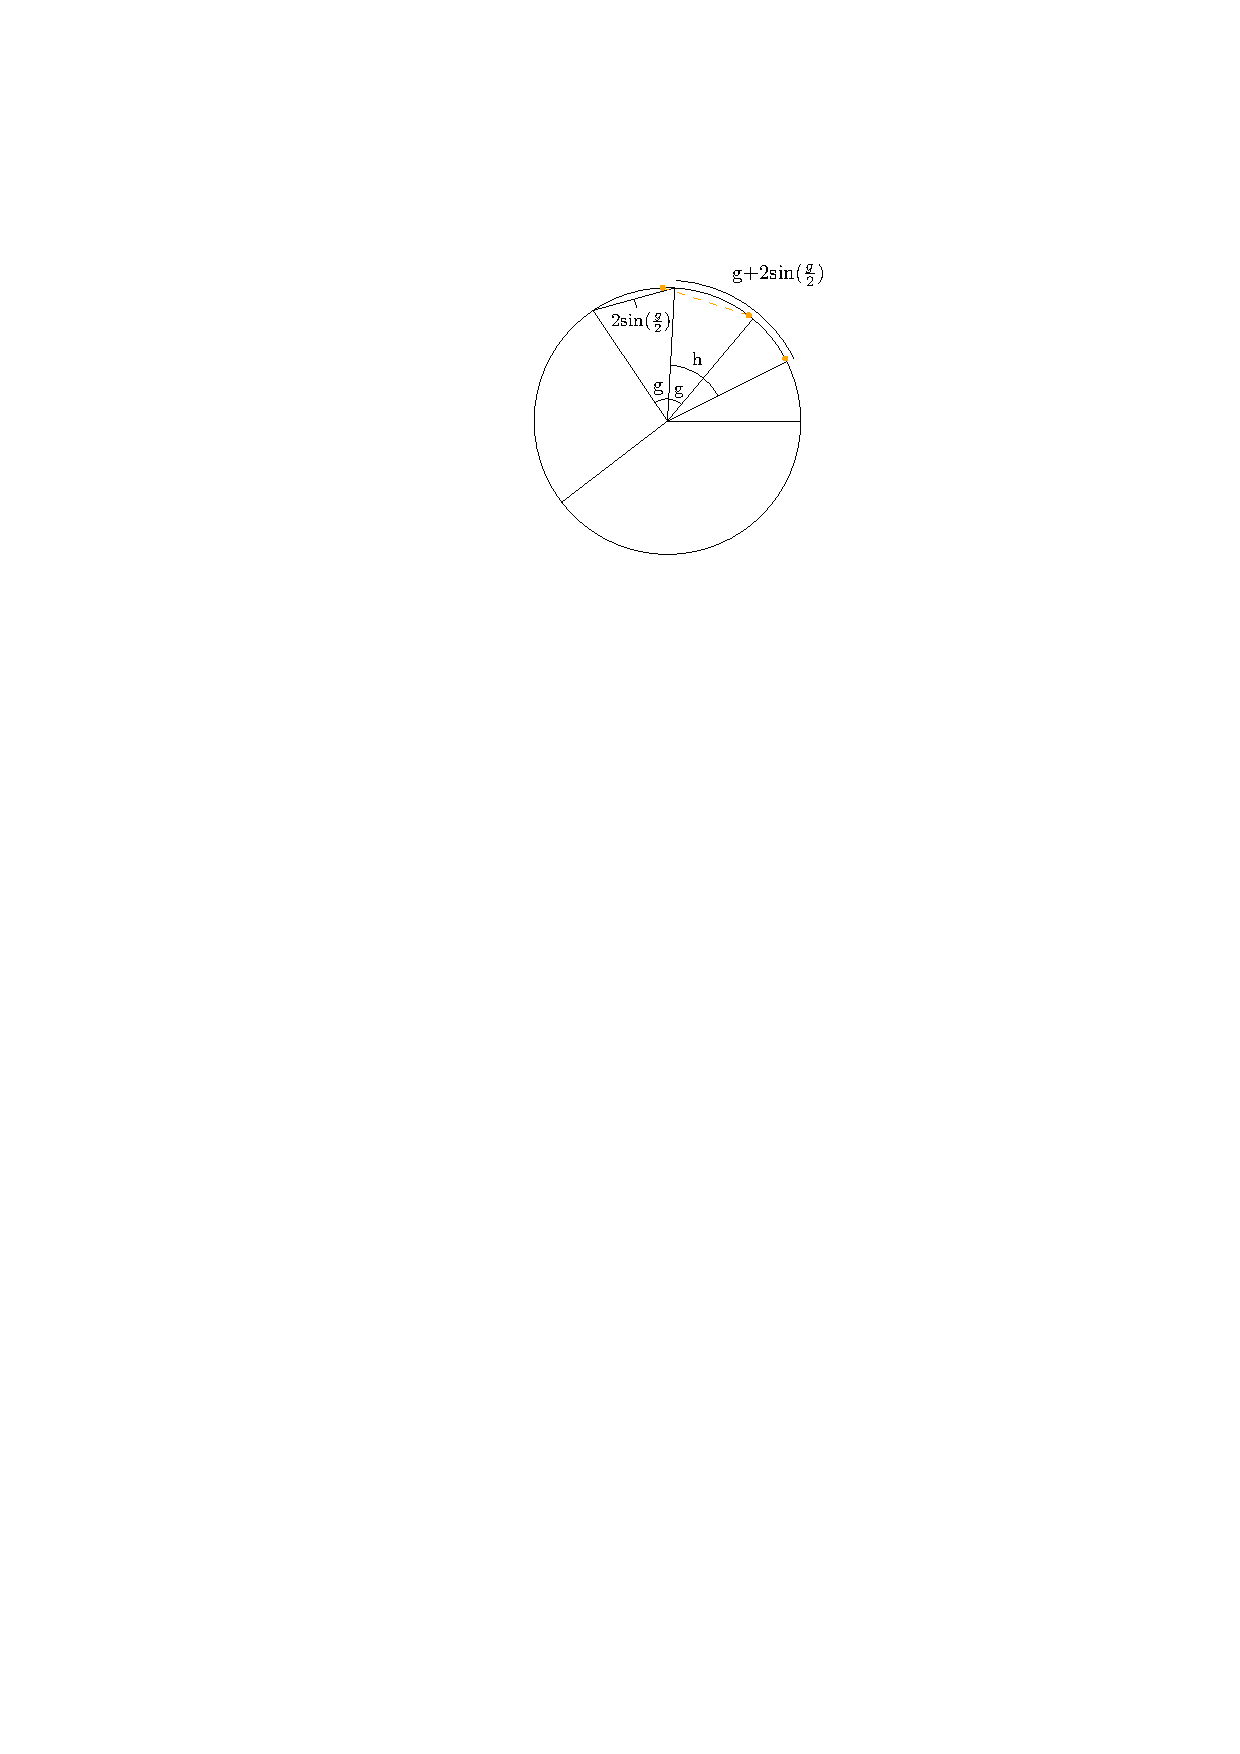
\includegraphics[width=0.25\textwidth]{Q2S1_Eq/ub_2.pdf}} \\
    \end{tabularx}

    Finally, a third bound gets introduced if $H$ finds the exit at a point such that both
    $P1$ and $P2$ are equidistant from $H$. For the time before the exit is found at this point of equal
    distance, evacuation is the responsibility of $P1$, and after this time, it is the responsibility
    of $P2$. The bound will occur after all the agents have travelled for $c+x$ time, and by this point,
    $P2$ will have begun its detour. The point of equidistance occurs when $P1$ and $H$ are
    $2\sin(c+x)$ apart, and as such the distance from $P2$'s point inside the circle to $H$'s point on
    the perimeter is the same.

    \begin{tabularx}{\textwidth}{p{0.4\textwidth}l}
        \multirow{2}{*}{$2\sin(c+x) =
        \sqrt{2}\sqrt{(x-1)\cos(g+h+x) - x\cos(g+x) -
        (x-1)x\cos(h) + (x-1)x + 1}$} & \\
    \end{tabularx}

\end{flushleft}

\end{document}
